\documentclass[conference]{IEEEtran}
    \IEEEoverridecommandlockouts
    % The preceding line is only needed to identify funding in the first footnote. If that is unneeded, please comment it out.
    \usepackage{cite}
    \usepackage[portuges,brazil,english]{babel}
    \usepackage{amsmath,amssymb,amsfonts}
    \usepackage{algorithmic}
    \usepackage{graphicx}
    \usepackage{textcomp}
    \def\BibTeX{{\rm B\kern-.05em{\sc i\kern-.025em b}\kern-.08em
        T\kern-.1667em\lower.7ex\hbox{E}\kern-.125emX}}
    \begin{document}
    
    \title{Baseline - Automated Sokoban}
    
    \author{\IEEEauthorblockN{Ignácio Espinoso}
    \IEEEauthorblockA{
    169767 \\
    ignacioespinoso@gmail.com}
    \and
    \IEEEauthorblockN{José Vincente}
    \IEEEauthorblockA{
    RA \\
    email address}
    \and
    \IEEEauthorblockN{Lauro Cruz}
    \IEEEauthorblockA{
    RA \\
    email address}
    \and
    \IEEEauthorblockN{Matheus Mortatti}
    \IEEEauthorblockA{
    RA \\
    email address}}
    
    \maketitle
    
    \section{Introduction}
    
    Sokoban is a classic puzzle game \cite{b1}, in which the goal is to push boxes to specific locations on the map. Developing a robot capable of solving the puzzles proves to be a challenge, since the problem deals with a variable map with multiple boxes, the robot must avoid reaching dead-ends and keep track of boxes positions.
    
    The developed baseline solution makes use of Open AI gym \cite{b2} and gym-sokoban \cite{b3} packages, which uses reinforcement Q-learning to solve the problem. \cite{b4}
    \begin{figure}[!htb]
    \begin{center}
    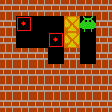
\includegraphics{pictures/Sokoban-small-v0.png}    
    \end{center}
    \caption{Sokoban Puzzle}
    \end{figure}
    
    \begin{thebibliography}{00}
    \bibitem{b1} https://en.wikipedia.org/wiki/Sokoban 
    \bibitem{b2} https://github.com/openai/gym 
    \bibitem{b3} https://github.com/mpSchrader/gym-sokoban
    \bibitem{b4} https://www.learndatasci.com/tutorials/reinforcement-q-learning-scratch-python-openai-gym/
    
    \end{thebibliography}
    
    \end{document}
    